\documentclass{article}
\usepackage[T1]{fontenc}
\usepackage{lmodern}
\usepackage{graphicx}
\usepackage{amsmath,amssymb}
\usepackage[a4paper,margin=2cm]{geometry}
\usepackage[absolute,overlay]{textpos}
\setlength{\TPHorizModule}{1mm}
\setlength{\TPVertModule}{1mm}
\usepackage[indonesian]{babel}
\usepackage{hyperref}
\setlength{\emergencystretch}{2em}
% unit: Halaman 28

\begin{document}

% === Halaman 28 (python/native) ===

3. Penyusup (intruder) 

      - Pihak ketiga yang menyadap, mengintersepsi, menghapus, menambah, atau 

          mengubah pesan

       - Sebutan lain: eavesdropper, enemy, adversary, interceptor, bad guy, dsb

       - Nama tokohnya: Eve, Carol, Trudy, Mallory, dsb 


28

Ronald Rivest: “cryptography is about communication in the presence of adversaries”

% deskripsi: gambar native xref 149
\noindent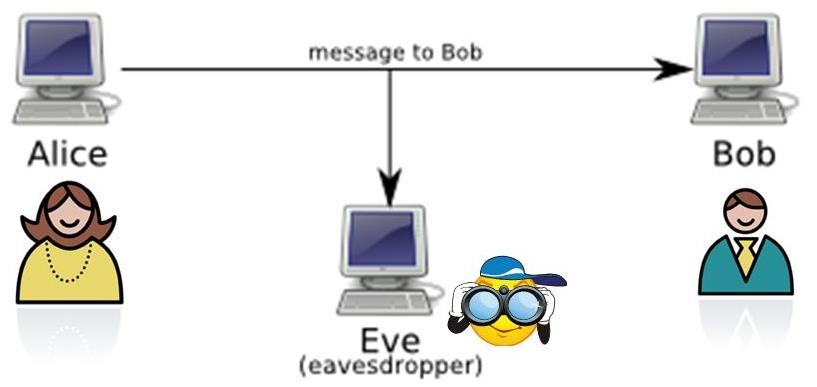
\includegraphics[width=0.85\textwidth]{../../images/python/page_028_img_01.jpeg}

\end{document}
